\section{Experimentos}
Realizamos experimentos para responder às seguintes perguntas:
\begin{enumerate}
\item \rqone
\item \rqtwo
\item \rqthree
\end{enumerate}

Foram implementados scripts em BASH para controlar os experimentos e fazer
medições, gerando arquivos .raw de saída contendo resultados. Foram também
implementados scripts em R que desenham gráficos de acordo com os arquivos .raw
gerados pelos scripts BASH.


Todos os experimentos foram realizados em uma máquina com processador Intel Core
i5 2.6Ghz e 8Gb de RAM. Cada medição de tempo nos experimentos foi realizada 10
vezes, e somente a média foi considerada e reportada nos resultados.
Todos os scripts e resultados estão disponíveis no diretório experiments.

\subsection{\rqone}
Nós comparamos a nossa implementação do LZ78 com o gzip em dois aspectos: Tempo
e taxa de compressão.
Para realizar essa comparação, nós escolhemos 11 arquivos de tamanhos distintos:
100KB, 200KB, 300KB, 700KB, 1MB, 2MB, 3MB, 5MB, 50MB e 1GB.
Todos os arquivos continham somente textos em inglês.

\subsubsection{Tempo}

Abaixo está um gráfico que relaciona o tempo que leva para comprimir um arquivo
com o tamanho dele, para ambos o nosso LZ78 e o gzip.
\\
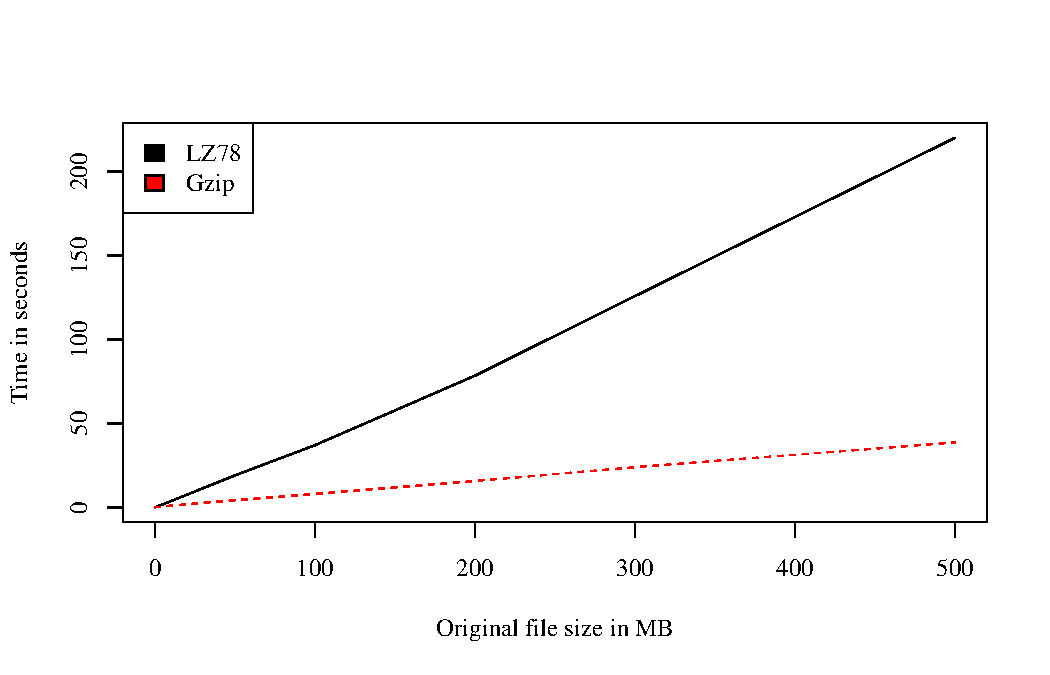
\includegraphics[scale=0.74]{../experiments/R/pdf/time_comp}
\\

Ambas as funções são (ou se aproximam muito de) retas, o que comprova que a
nossa implementação do \lz, bem como o \gzip, acontecem em tempo linear de
acordo com o tamanho do arquivo. Porém, a constante que multiplica a função do
\gzip é bem menor do que a nossa. Isso acontece porque o \gzip está em
desenvolvimento a mais de 23 anos, onde experts estão sempre otimizando o
algoritmo, fazendo com que essa constante da função linear seja cada vez menor.

\subsubsection{Taxa de compressão}

Abaixo está um gráfico que relaciona a taxa de compressão de um  arquivo com o
tamanho dele, para ambos o nosso \lz e o \gzip.
\\
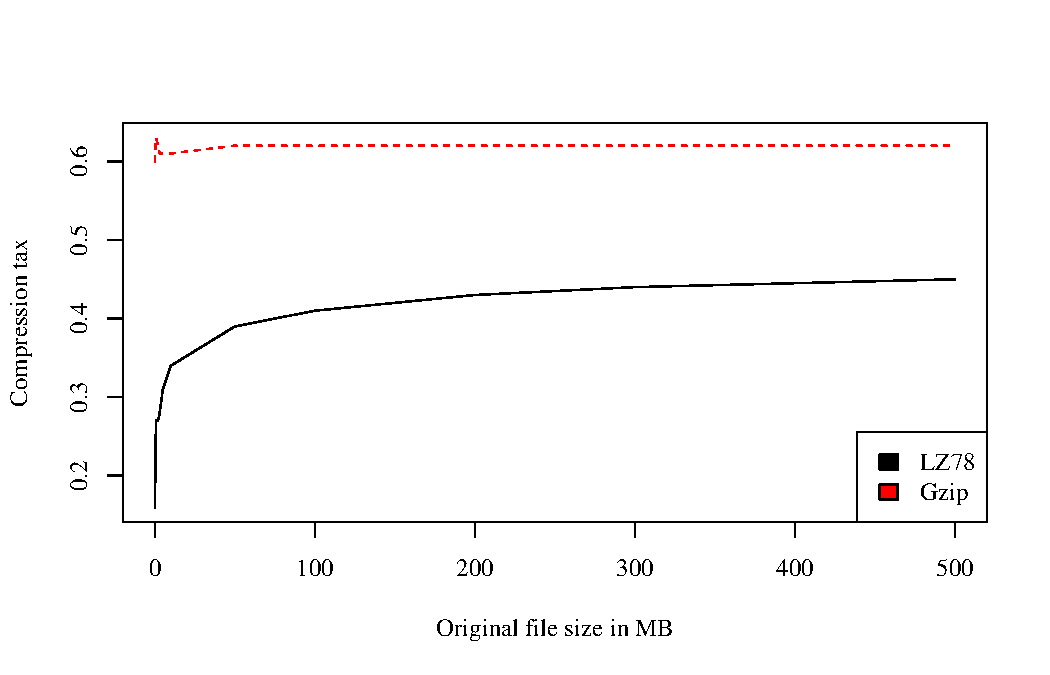
\includegraphics[scale=0.74]{../experiments/R/pdf/comp_tax}
\\


